\chapter{Einleitung}
\label{sec:Einleitung}

\section{Motivation}
\label{sec:Motivation}
Das Mooresche Gesetz aus den 60iger Jahren sagt aus, dass sich die Zahl der Transistoren auf integrierten Schaltungen alle 18 Monate verdoppelt. Dies wirkt sich auch analog auf die Rechenleistung aus. In den letzten Jahren wird die Erhöhung der Rechenleistung allerdings nicht mehr durch noch schnellere Prozessoren erzielt, sondern durch den Einsatz von mehreren Prozessorkernen, die dann eine Einheit bilden und (echte) parallele Verarbeitung ermöglichen.

Während bei der Verbesserung der Ein-Kern-Prozessoren die Datenbanksysteme ebenso direkt davon profitieren konnten, stellen sich bei Multicore-Prozessoren neue Herausforderungen an das Datenbanksystem. Um das komplette Potenzial der Multicore-Prozessoren ausreizen zu können, müssen Algorithmen angepasst und neu erfunden werden.

\section{Ziele der Arbeit}
\label{sec:ZieleDerArbeit}
In dieser Arbeit werden verschiedene Ansätze vorgestellt, wie Datenbanken und deren Algorithmen modifiziert werden können, um das volle Potenzial von Multicoreprozessoren auszunutzen. Dabei soll an verschiedenen Punkten angesetzt werden. Ein Datenbankmanagementsystem besitzt klassischerweise fünf Schichten (siehe Abbildung \ref{fig:dbschichten}). Mit der Auswahl der Algorithmen versuchen wir möglichst viele dieser Schichten abzudecken.

\begin{figure}[htb]
	\begin{center}
        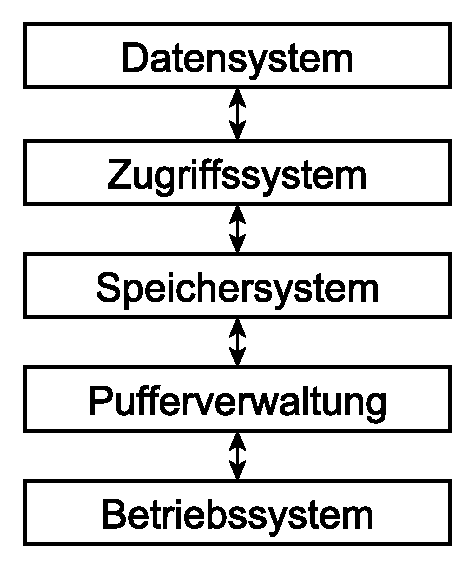
\includegraphics[scale=0.5]{Bilder/dbschichten.pdf}  
    	\textsf{\caption{Schichten eines Datenbanksystems}\label{fig:dbschichten}}
		
	\end{center}
\end{figure}

Der MCC-DB Algorithmus arbeitet auf Daten- und Betriebssystem, wobei der Hauptaugenmerk auf Betriebssystemebene liegt. AA-Hash-Join und Aligned Access Sort optimieren auf Schicht des Zugriffssystems und Parallel SQL Auto-Tuning versucht nur auf Datensystem-Ebene zu verbessern.

Das Ziel ist nun diese Algorithmen zu untersuchen und miteinander in Ihrer Effizienz und ihrem Aufwand zu vergleichen.

\section{Aufbau der Arbeit}
\label{sec:AufbauDerArbeit}
Im zweiten Kapitel werden die Grundlagen und Grundbegriffe über die Themen Multicoreprozessoren und Datenbank erläutert, damit jeder Leser den Ausführungen im Kapitel drei folgen kann. Im dritten Kapitel werden aktuelle Ansätze zur Optimierung der Datenbanken auf Multicoreprozessoren vorgestellt und anschließend auch bewertet. Dabei betrachten wir Optimierungen im Cache, am Zugriffsplan und bei Join- und Sort-Algorithmen. Das letzte Kapitel enthält eine Zusammenfassung unserer Erkenntnisse und gibt noch einen weiteren Ausblick auf weitere Ansätze in verwandten Themengebieten.